% SLIDE 1: pagina di presentazione
\frame{\titlepage}

% SLIDE 2: motivazioni
\begin{frame}
    \frametitle{Scenario e Motivazioni}
    Il mondo del Cloud ha portato molti benefici, tuttavia solleva diverse problematiche legate alla \alert{mancanza di fiducia}
    \hfill\break
    \begin{itemize}
        \item Non vengono fornite agli utenti le specifiche riguardanti le misure di sicurezza messe in atto
        \item Sono sistemi specifici e \alert{difficili da utilizzare} se non si ha esperienza in materia
    \end{itemize}
\end{frame}

% SLIDE 3: motivazioni (2)
\begin{frame}
    \frametitle{Scenario e Motivazioni (2)}
    \begin{columns}
        \begin{column}{0.55\textwidth}
            Moon Cloud è una piattaforma erogata come servizio, la quale supporta:
            \begin{itemize}
                \item Un sistema di \textit{Security Governance}
                \item Un framework di \alert{\textit{Security Assurance}}
            \end{itemize}
        \end{column}
        \begin{column}{0.4\textwidth}
            \begin{center}
                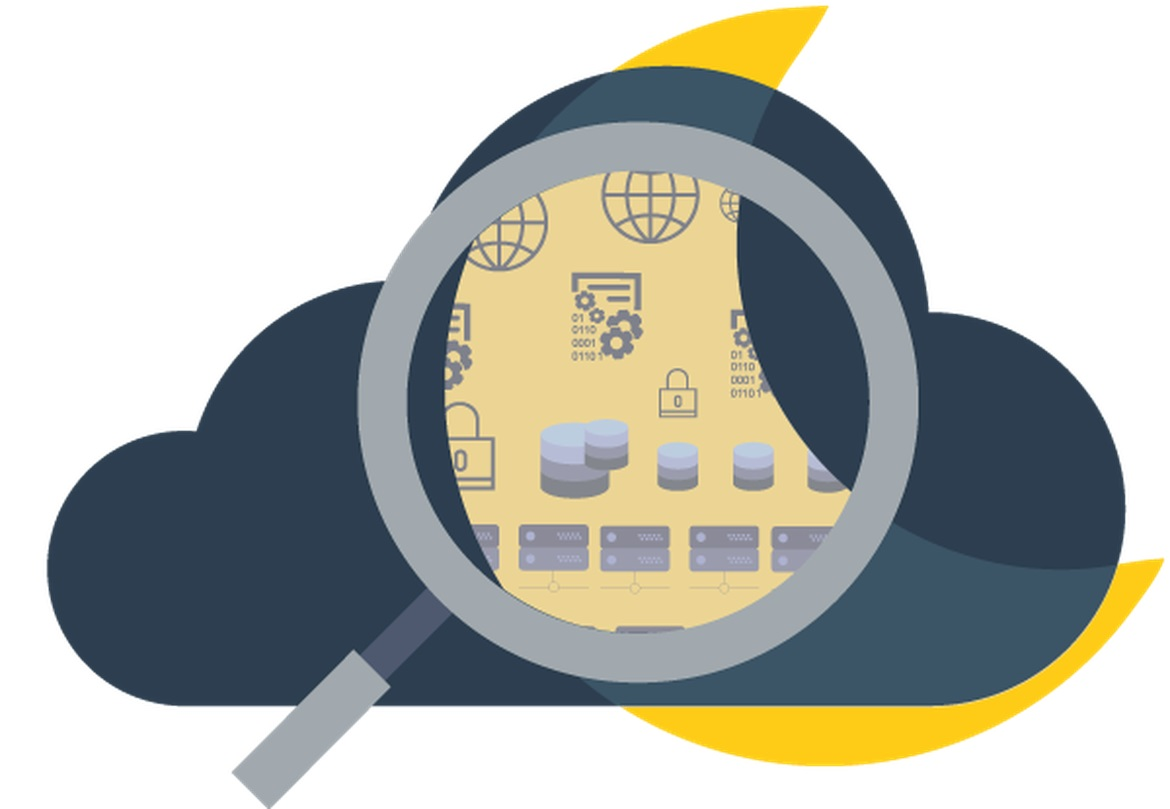
\includegraphics[scale=0.12]{images/mc}
            \end{center}
        \end{column}
    \end{columns}
    Garantisce il controllo della sicurezza informatica in modo rapido ed efficiente, attraverso attività di test e monitoraggio 
    periodiche e programmate
\end{frame}

% SLIDE 4: obiettivi
\begin{frame}
    \frametitle{Obiettivo della tesi}
    Introdurre un \alert{sistema di raccomandazione} che possa consigliare all'utente delle possibili \textit{Evaluation} rispetto 
    all'\textit{asset} che si vuole proteggere e monitorare
    \begin{itemize}
        \item L'utente meno esperto può usufruire dei servizi offerti da Moon Cloud in modo \alert{semplice} e \alert{intuitivo}
        \item Si è cercato di colmare il problema della mancata fiducia in questi sistemi
    \end{itemize}
\end{frame}

% SLIDE 5: sistema di raccomandazione
\begin{frame}
    \frametitle{Sistema di raccomandazione}
    Un \textit{recommendation system} può filtrare i dati usando differenti algoritmi e raccomandare gli item più rilevanti agli utenti attraverso 
    un procedimento a 3 fasi
    \begin{enumerate}
        \item \alert{Raccolta di dati}: ottenere informazioni rilevanti e consistenti su cui applicare algoritmi di raccomandazione
        \item \alert{Memorizzazione di dati}: la quantità di dati definisce quanto efficace un modello di raccomandazione può di diventare
        \item \alert{Filtraggio dei dati}: estrarre le informazioni più rilevanti
    \end{enumerate}
\end{frame}

% SLIDE 6: Collaborative Filter
\begin{frame}
    \frametitle{Collaborative filtering}
    Questo sistema predice la preferenza che un utente accorderebbe a un item basandosi sulle preferenze date da altri utenti
    \begin{itemize}
        \item Memory-based: metodi che mirano a determinare il grado di relazione tra utenti e item identificando 
        utenti con uno storico di item usati simile
            \begin{itemize}
                \item \alert{UB-CF}: algoritmo che fornisce dei suggerimenti sulla base di uno o più vicini (\textit{neighbours})
                \item \alert{IB-CF}: algoritmo che confronta gli item dell'utente a cui si vuole raccomandare e i possibili item simili
            \end{itemize}
        \item Hybrid filter: combinazione di più tecniche di raccomandazione per raggruppare i pregi di ciascun approccio
    \end{itemize}
\end{frame}

% SLIDE 7: Collaborative Filter (2)
\begin{frame}
    \frametitle{Collaborative filtering (2)}
    \begin{columns}
        \begin{column}{0.5\textwidth}
            \begin{figure}
                \centering
                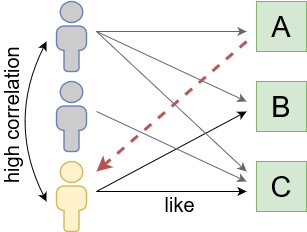
\includegraphics[scale=0.5]{images/UB_CF_ex}
                %\caption{User based Collaborative Filter}
            \end{figure}
        \end{column}
        \begin{column}{0.5\textwidth}
            \begin{figure}
                \centering
                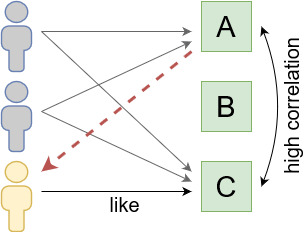
\includegraphics[scale=0.5]{images/IB_CF_ex}
                %\caption{Item based Collaborative Filter}
            \end{figure}
        \end{column}
    \end{columns}
\end{frame}

% SLIDE 8: Soluzione
\begin{frame}
    \frametitle{Soluzione}
    Servizio di \alert{API REST}, che si appoggia a un database Postgres, accessibile 
    attraverso apposite URL; questo servizio permette di effettuare richieste al sistema di raccomandazione e di aggiornare la base di dati
    \begin{enumerate}
        \item Preparazione della base di dati
        \item Realizzazione delle View
        \item Consistenza tra i database
        \item Deployment in Docker
    \end{enumerate}
\end{frame}

% SLIDE 9: Soluzione (2)
\begin{frame}
    \frametitle{Soluzione (2)}
    \begin{figure}
        \centering
        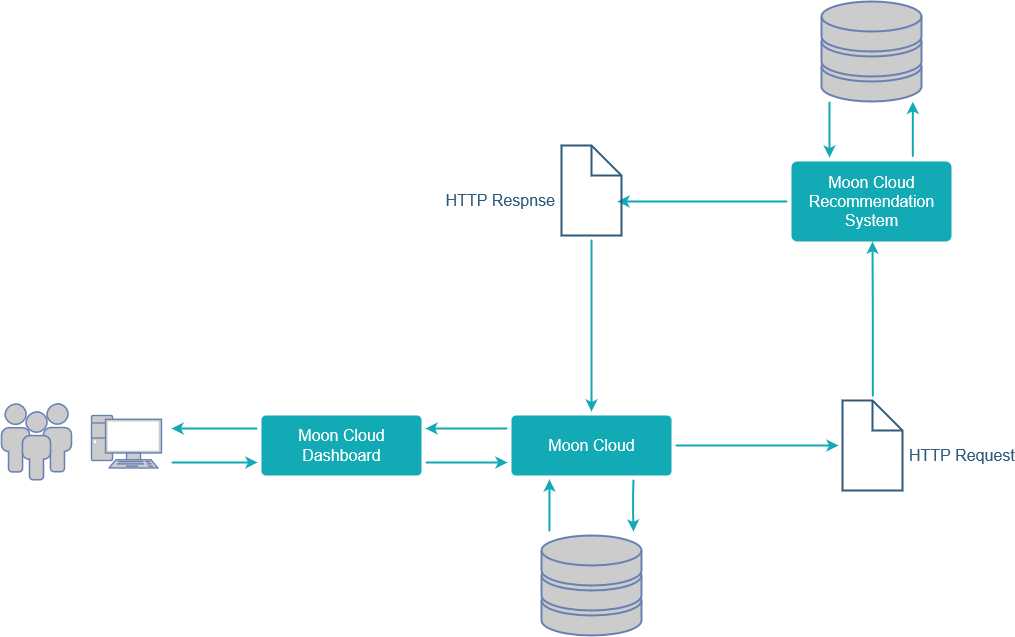
\includegraphics[scale=0.42]{images/UML_MoonCloud_HowToDo}
    \end{figure}
\end{frame}

% SLIDE 10: Conclusioni
\begin{frame}
    \frametitle{Conclusioni}
    La soluzione proposta introduce un sistema di raccomandazione in un mondo in cui spesso non è presente perché 
    popolato da utenti esperti
    \begin{itemize}
        \item Viene data una possibilità a un \alert{maggior numero di utenti} di accedere a servizi su un sistema Cloud di 
        Security Assurance in totale sicurezza e affidabilità
    \end{itemize}
\end{frame}

% SLIDE 11:
%\begin{frame}
%    \frametitle{}

%\end{frame}

% SLIDE 12:
%\begin{frame}
%    \frametitle{}

%\end{frame}
